\documentclass[10pt,a4paper]{article}
\usepackage[utf8]{inputenc}
\usepackage[margin=0.6in]{geometry}
\usepackage{graphicx}
\usepackage{microtype}
\usepackage{titlesec}
\usepackage{hyperref}
\usepackage{booktabs}
\usepackage{enumitem}
\usepackage{xcolor}
\usepackage{tabularx}

\graphicspath{{certificates/}{./}}

\definecolor{amritablue}{RGB}{0, 51, 102}
\definecolor{darkgray}{RGB}{50, 50, 50}

\hypersetup{
    colorlinks=true,
    linkcolor=amritablue,
    urlcolor=amritablue,
}

\titlespacing*{\section}{0pt}{4pt}{2pt}
\titlespacing*{\subsection}{0pt}{3pt}{1pt}

\titleformat{\section}
  {\normalfont\small\bfseries\color{amritablue}\uppercase}
  {\thesection}{1em}{}[\titlerule]

\setlist{nosep, leftmargin=13pt}

\begin{document}
\pagestyle{empty}

% =========================================================
% PAGE 1: COURSE COMPLETION CERTIFICATE
% =========================================================
\begin{center}
    {\large\textbf{\color{amritablue}AMRITA VISHWA VIDYAPEETHAM}}\\[1pt]
    {\footnotesize\textbf{Amrita School of Computing, Coimbatore --- Department of Computer Science and Engineering}}\\[2pt]
    {\footnotesize\textbf{Technical Enrichment Activity: Professional Online Certification (20 Marks)}}\\[1pt]
    {\scriptsize Official Course Completion Certificate}
\end{center}

\vspace{-4pt}
\hrule height 0.8pt
\vspace{6pt}

\noindent
\begin{tabularx}{\textwidth}{@{}l X l X@{}}
    \textbf{Student Name:} & Chitturi Vivek Vardhan & \textbf{Course Title:} & Supervised Machine Learning: Regression and Classification \\
    \textbf{Roll Number:} & CB.SC.U4CSE23360 & \textbf{Platform / Provider:} & Coursera / DeepLearning.AI \& Stanford Online \\
    \textbf{Degree \& Branch:} & B.Tech CSE (VII Semester) & \textbf{Project Guide:} & Ms. Neethu M R (Asst. Professor) \\
\end{tabularx}

\vspace{12pt}
\begin{center}
    \fbox{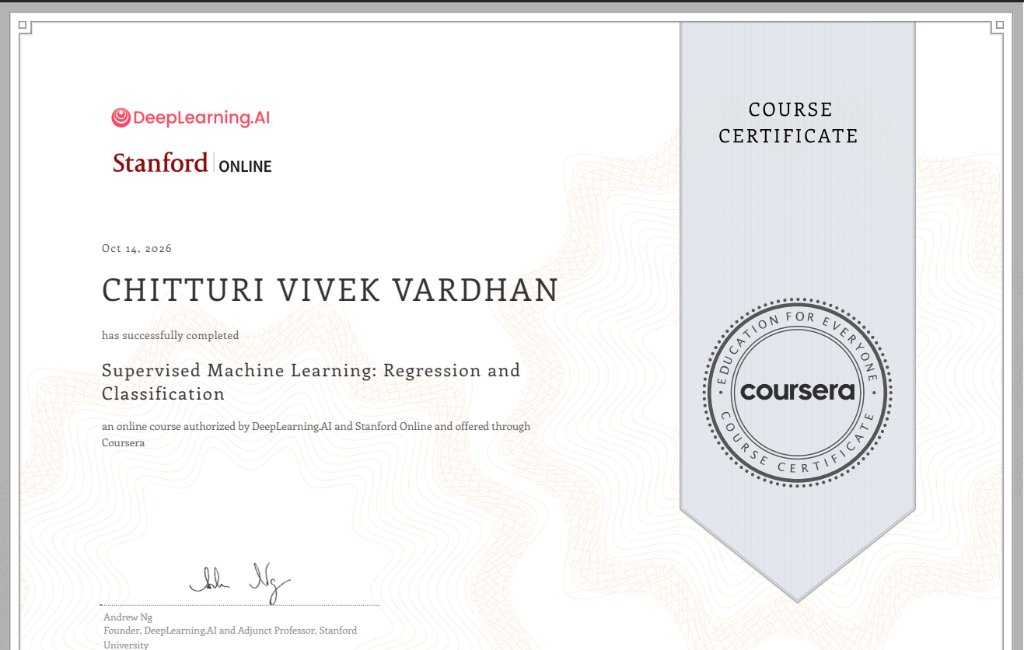
\includegraphics[width=0.96\textwidth, height=0.70\textheight, keepaspectratio]{vivek_cert.png}}
\end{center}

\vfill
\begin{center}
    {\footnotesize\textbf{Course Authorization:} DeepLearning.AI \& Stanford Online --- Instructor: Andrew Ng}
\end{center}

\clearpage

% =========================================================
% PAGE 2: TECHNICAL ALIGNMENT REPORT
% =========================================================
\begin{center}
    {\large\textbf{\color{amritablue}AMRITA VISHWA VIDYAPEETHAM}}\\[1pt]
    {\footnotesize\textbf{Amrita School of Computing, Coimbatore --- Department of Computer Science and Engineering}}\\[2pt]
    {\footnotesize\textbf{Technical Enrichment Activity: Professional Online Certification (20 Marks)}}\\[1pt]
    {\scriptsize Course Completion Details \& One-Page Technical Alignment Report}
\end{center}

\vspace{-4pt}
\hrule height 0.8pt
\vspace{4pt}

\noindent
\begin{tabularx}{\textwidth}{@{}l X l X@{}}
    \textbf{Student Name:} & Chitturi Vivek Vardhan & \textbf{Course Title:} & Supervised Machine Learning: Regression and Classification \\
    \textbf{Roll Number:} & CB.SC.U4CSE23360 & \textbf{Platform / Provider:} & Coursera / DeepLearning.AI \& Stanford Online \\
    \textbf{Degree \& Branch:} & B.Tech CSE (VII Semester) & \textbf{Duration / Effort:} & 15--20 Hours (10--20 Hour Category) \\
    \textbf{Project Guide:} & Ms. Neethu M R (Asst. Professor) & \textbf{Course Instructor:} & Andrew Ng (Stanford Adjunct Professor) \\
\end{tabularx}

\vspace{3pt}
\noindent
\textbf{B.Tech Project Title:} \textit{EdgeTrust-VANET: A Decentralized Trust Management and Machine Learning Framework for Secure Vehicular Ad Hoc Networks}

\vspace{2pt}
\section*{1. Course Curriculum \& Technical Competencies Acquired}
The certification \textit{Supervised Machine Learning: Regression and Classification} (Stanford Online and DeepLearning.AI via Coursera) covers foundational statistical learning, predictive modeling, and optimization algorithms:
\begin{itemize}
    \item \textbf{Supervised Classification Formulations:} Linear and logistic regression architectures, sigmoid activation, decision boundary geometry, and binary cross-entropy cost functions.
    \item \textbf{Gradient Descent \& Numerical Optimization:} Batch gradient descent, learning rate scheduling, vectorization, and numerical stability in multi-feature spaces.
    \item \textbf{Overfitting Mitigation \& Regularization:} Mathematical formulation of L1/L2 weight penalties, bias-variance tradeoff analysis, and feature scaling.
    \item \textbf{Model Evaluation under Class Imbalance:} Precision, recall, F1-score optimization, receiver operating characteristic (ROC-AUC), and confusion matrix diagnostics.
\end{itemize}

\section*{2. Technical Justification: How the Course Directly Supports EdgeTrust-VANET}
In EdgeTrust-VANET, vehicles broadcast Basic Safety Messages (BSMs) at 10~Hz, requiring immediate, high-confidence classification between benign nodes and malicious adversaries injecting fabricated kinematics. The supervised learning principles mastered in this course directly underpinned our machine learning design, training pipeline, and empirical evaluation:

\begin{enumerate}
    \item \textbf{Mathematical Formulation of Vehicular Misbehavior Detection:} 
    Using the binary classification paradigms taught in the course, we formulated insider anomaly detection as a predictive classification task ($y \in \{0, 1\}$) across 15 standardized VeReMi attack behaviors (including position spoofing, sudden deceleration illusions, and stealthy adaptive trajectory drifts).

    \item \textbf{Sub-Microsecond Linear Classifier Design (Tier 1 / Tier 2 Pre-Filter):} 
    Guided by the course's logistic regression framework and vectorized matrix mathematics, we engineered a natively compiled C++ linear classifier with L2 regularization. Executing in just \textbf{0.38~$\mu$s} per message with a 91.20\% baseline accuracy and an ultra-compact 0.8~KB footprint, this model serves as an instantaneous pre-filter for resource-constrained edge gateways.

    \item \textbf{Loss Function Optimization \& Combating Class Imbalance:} 
    In real vehicular streams, benign transmissions vastly outnumber insider attack packets. Applying the course's cost-function weighting and probability threshold tuning, we calibrated decision boundaries to penalize false alarms, directly contributing to slashing our system False Positive Rate from 12.42\% down to \textbf{1.85\%} while achieving a peak F1-score of \textbf{97.28\%}.

    \item \textbf{Feature Normalization \& 14-Dimensional Space Partitioning ($\mathbf{x} \in \mathbb{R}^{14}$):} 
    The course's principles on feature scaling and gradient descent convergence enabled the effective fusion of disparate physical kinematic dimensions (velocity residuals, acceleration bounds) and dynamic Bayesian trust metrics into a normalized 14-dimensional feature vector.
\end{enumerate}

\section*{3. Measurable Project Outcomes Supported by this Certification}
\noindent
\begin{tabularx}{\textwidth}{@{}X X X@{}}
    \textbf{Model F1-Score:} 97.28\% (Precision: 98.15\%) & 
    \textbf{Pre-Filter Latency:} 0.38~$\mu$s execution time & 
    \textbf{Academic Status:} IEEE Conference Paper Under Review \\
\end{tabularx}

\end{document}
